\let\negmedspace\undefined
\let\negthickspace\undefined
\documentclass[journal]{IEEEtran}
\usepackage[a5paper, margin=10mm, onecolumn]{geometry}
%\usepackage{lmodern} % Ensure lmodern is loaded for pdflatex
\usepackage{tfrupee} % Include tfrupee package

\setlength{\headheight}{1cm} % Set the height of the header box
\setlength{\headsep}{0mm}  % Set the distance between the header box and the top of the text

\usepackage{gvv-book}
\usepackage{gvv}
\usepackage{cite}
\usepackage{amsmath,amssymb,amsfonts,amsthm}
\usepackage{algorithmic}
\usepackage{graphicx}
\usepackage{textcomp}
\usepackage{xcolor}
\usepackage{txfonts}
\usepackage{listings}
\usepackage{enumitem}
\usepackage{mathtools}
\usepackage{gensymb}
\usepackage{comment}
\usepackage[breaklinks=true]{hyperref}
\usepackage{tkz-euclide} 
\usepackage{listings}
% \usepackage{gvv}                                        
\def\inputGnumericTable{}                                 
\usepackage[latin1]{inputenc}                                
\usepackage{color}                                            
\usepackage{array}                                            
\usepackage{longtable}                                       
\usepackage{calc}
\usepackage{caption}
\usepackage{multirow}                                         
\usepackage{hhline}                                           
\usepackage{ifthen}                                           
\usepackage{lscape}
\usepackage{tikz}
\usetikzlibrary{patterns}
\begin{document}

\bibliographystyle{IEEEtran}
\vspace{3cm}


\title{GATE 2021 ES}
\author{ee25btech11035 - Kushal B N}
\maketitle
% \maketitle
% \newpage
% \bigskip
{\let\newpage\relax\maketitle}

% \renewcommand{\thefigure}{\theenumi}
\renewcommand{\thetable}{\theenumi}
\setlength{\intextsep}{10pt} % Space between text and floats



\section{General Aptitude (GA)}
Q.1 - Q.5 Multiple Choice Question (MCQ), carry ONE mark each (for each wrong answer: -1/3)
\bigskip
\begin{enumerate}[start=1]
	\item The current population of a city is 11,02,500. If it has been increasing at the rate of 5\% per annum, what was its population 2 years ago?
    \hfill\brak{GATE~ES~2021}
\begin{enumerate}
\begin{multicols}{2}
\item 9,92,500
\item 9,95,006
\item 10,00,000
\item 12,51,506
\end{multicols}
\end{enumerate}

\item  $p$ and $q$ are positive integers and  $\frac{p}{q} + \frac{q}{p} = 3,$ then, $\frac{p^2}{q^2} + \frac{q^2}{p^2}$
\hfill\brak{GATE~ES~2021}
\begin{enumerate}
\begin{multicols}{4}
\item 3
\item 7
\item 9
\item 11
\end{multicols}
\end{enumerate}

\setcounter{figure}{0}
\begin{figure}[H]
    \centering
    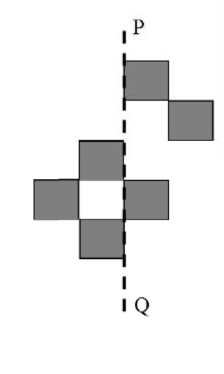
\includegraphics[width=0.3\columnwidth]{figs/image_1.png}
    \caption{Figure for Q.3}
    \label{Figure1}
\end{figure}

\item The least number of squares that must be added so that the line P-Q becomes the line of symmetry is \_\_\_\_\_\_
\hfill\brak{GATE~ES~2021}
\begin{enumerate}
\begin{multicols}{4}
\item 4
\item 3
\item 6
\item 7
\end{multicols}
\end{enumerate}

\item \textit{Nostalgia} is to \textit{anticipation} as \_\_\_\_\_\_ is to \_\_\_\_\_\_ \\
Which one of the following options maintains a similar logical relation in the above sentence?
\hfill\brak{GATE~ES~2021}
\begin{enumerate}
\begin{multicols}{2}
\item Present, past
\item Future, past
\item Past, future
\item Future, present
\end{multicols}
\end{enumerate}

\item Consider the following sentences:
\begin{enumerate}[label=(\roman*)]
    \item I woke up from sleep.
    \item I woked up from sleep.
    \item I was woken up from sleep.
    \item I was wokened up from sleep.
\end{enumerate}
Which of the above sentences are grammatically CORRECT?
\hfill\brak{GATE~ES~2021}
\begin{enumerate}
\begin{multicols}{2}
\item (i) and (ii)
\item (i) and (iii)
\item (ii) and (iii)
\item (i) and (iv)
\end{multicols}
\end{enumerate}

Q.6 - Q.10 Multiple Choice Question (MCQ), carry TWO marks each (for each wrong answer: -2/3).\\

\item Given below are two statements and two conclusions.\\
Statement 1: All purple are green.\\
Statement 2: All black are green.\\
Conclusion I: Some black are purple.\\
Conclusion II: No black is purple.\\
Based on the above statements and conclusions, which one of the following options is logically CORRECT?
\hfill\brak{GATE~ES~2021}
\begin{enumerate}
\item Only conclusion I is correct.
\item Only conclusion II is correct.
\item Either conclusion I or II is correct.
\item Both conclusion I and II are correct.
\end{enumerate}


\item 
Computers are ubiquitous. They are used to improve efficiency in almost all fields from agriculture to space exploration. Artificial intelligence (AI) is currently a hot topic. AI enables computers to learn, given enough training data. For humans, sitting in front of a computer for long hours can lead to health issues.\\
Which of the following can be deduced from the above passage?\\
(i) Nowadays, computers are present in almost all places.\\
(ii) Computers cannot be used for solving problems in engineering.\\
(iii) For humans, there are both positive and negative effects of using computers.\\
(iv) Artificial intelligence can be done without data.
\hfill\brak{GATE~ES~2021}
\begin{enumerate}
\begin{multicols}{2}
\item (ii) and (iii)
\item (ii) and (iv)
\item (i), (iii) and (iv)
\item (i) and (iii)
\end{multicols}
\end{enumerate}

\item Consider a square sheet of side 1 unit. In the first step, it is cut along the main diagonal to get two triangles. In the next step, one of the cut triangles is revolved about its short edge to form a solid cone. The volume of the resulting cone, in cubic units, is \_\_\_\_\_\_\_
\hfill\brak{GATE~ES~2021}
\begin{enumerate}
\begin{multicols}{4}
\item $\frac{\pi}{3}$
\item $\frac{2\pi}{3}$
\item $\frac{3\pi}{2}$
\item $3\pi$
\end{multicols}
\end{enumerate}

\item 
\begin{figure}[H]
    \centering
    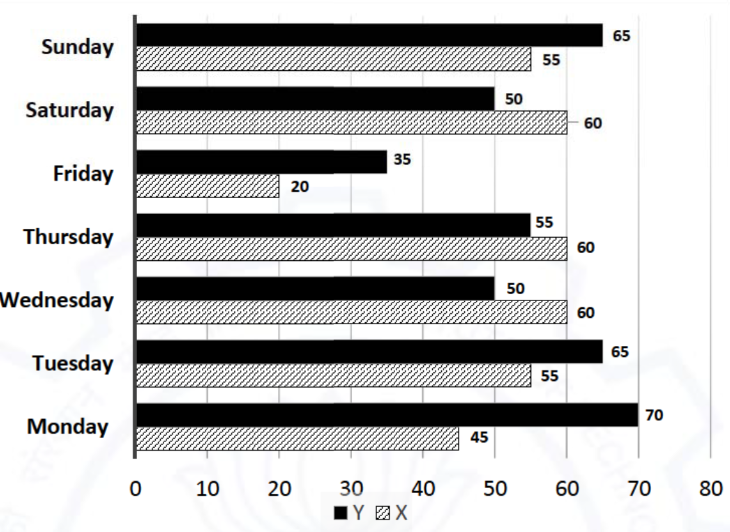
\includegraphics[width=0.5\columnwidth]{figs/image_2.png}
    \caption{Bar Chart for Q.9}
    \label{figure2}
\end{figure}
The number of minutes spent by two students, $X$ and $Y$, exercising every day in a given week are shown in the \figref{figure2} above.\\
The number of days in the given week in which one of the students spent a minimum of 10\% more than the other student, on a given day, is
\hfill\brak{GATE~ES~2021}
\begin{enumerate}
\begin{multicols}{4}
\item 4
\item 5
\item 6
\item 7
\end{multicols}
\end{enumerate}

\item 
\begin{figure}[H]
    \centering
    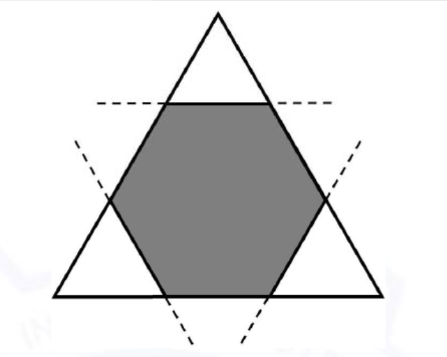
\includegraphics[width=0.5\columnwidth]{figs/image_3.png}
    \caption{Figure for Q.10}
    \label{figure3}
\end{figure}
Corners are cut from an equilateral triangle to produce a regular conved hexagon as shown in \figref{figure3}.\\
The ratio of the area of the regular convex hexagon to the area of the original equilateral triangle is
\hfill\brak{GATE~ES~2021}
\begin{enumerate}
\begin{multicols}{2}
\item 2 : 3
\item 3 : 4
\item 4 : 5
\item 5 : 6
\end{multicols}
\end{enumerate}

\end{enumerate}

\section{Environmental Science and Engineering(ES)}
\bigskip
Q.1 - Q.18 Multiple Choice Question (MCQ), carry ONE mark each (for each wrong answer: -1/3).
\bigskip

\begin{enumerate}[start=1]
\item A tangent is drawn on the curve of the funtion $y = x^2$ at the point $(x,y)=(3,9)$. The slope of the tangent is \_\_\_\_.
\hfill\brak{GATE~ES~2021}
\begin{enumerate}
\begin{multicols}{4}
\item 3
\item 6
\item 9
\item 12
\end{multicols}
\end{enumerate}

\item $\lim_{x \to 0}{\frac{x^2}{\sin{x}}}$
\hfill\brak{GATE~ES~2021}
\begin{enumerate}
\begin{multicols}{4}
\item 0
\item 1
\item 2
\item -1
\end{multicols}
\end{enumerate}

\item The table below shows the carbon content of four samples of powdered coal. If these four samples are mixed completely, what would be the resultant carbon percentage of the mixture by weight?

\begin{table}[h!]
\centering
\begin{tabular}{|c|c|c|}
\hline
Sample number & Mass of sample (kg) & Carbon \% by weight \\ \hline
1 & 2 & 88 \\ \hline
2 & 1 & 90 \\ \hline
3 & 2 & 80 \\ \hline
4 & 1 & 90 \\ \hline
\end{tabular}
\end{table}

\hfill\brak{GATE~ES~2021}
\begin{multicols}{4}
\begin{enumerate}
\item 58 \%
\item 86 \%
\item 87 \%
\item 90 \%
\end{enumerate}
\end{multicols}
\item A sample of air is collected in the morning at an ambient temperature of $25\celsius$. The concentration of carbon monoxide ($CO$) in this sample is 30 ppmv (ppm by volume). The same sample is analysed later in the afternoon when the sample temperature is $35\celsius$. The analysis results will show the $CO$ concentration as \_\_\_\_\_. 
\hfill\brak{GATE~ES~2021}
\begin{multicols}{4}
\begin{enumerate}
\item $<$ 29 ppmv
\item $>$ 30 ppmv
\item = 30 ppmv
\item = 29 ppmv

\end{enumerate}
\end{multicols}

\item In fluid statics, the line of action of the buoyant force \textit{always} acts through the \_\_\_\_\_.
\hfill\brak{GATE~ES~2021}
\begin{enumerate}
\item centre of gravuty of any submerged body
\item centroid of the volume of any floating body
\item centroid of the displaced volume of fluid by the body
\item centroid of the volume of fluid vertically above the body
\end{enumerate}

\item What is the order of preference of the various elements in integrated waste management hierarchy (highest preference to lowest preference)?
\hfill\brak{GATE~ES~2021}
\begin{enumerate}
\item Reduce $>$ Reuse \& recycle $>$ Energy recovery $>$ Landfilling
\item Reuse \& recycle $>$ Reduce $>$ Energy recovery $>$ Landfilling
\item Reduce $>$ Energy recovery $>$ Reuse \& recycle $>$ Landfilling
\item Reduce $>$ Reuse \& recycle $>$ Landfilling $>$ Energy recovery
\end{enumerate}

\item If $d$ is the depth of an quifier through which water is flowing, then the relationship between permeability $K$ and transmissibility (also known as transmissivity)$T$ is given by \_\_\_\_\_.
\hfill\brak{GATE~ES~2021}
\begin{multicols}{4}
\begin{enumerate}
\item $T = Kd$
\item $T = K/d$
\item $T = \sqrt{Kd}$
\item $K = \sqrt{Td}$
\end{enumerate}
\end{multicols}

\item Which of the following is the terminal electron acceptor in the electron transport chain of aerobic respiration?
\hfill\brak{GATE~ES~2021}
\begin{enumerate}
\item Water
\item NADH
\item $O_2$
\item Cytochrome-c
\end{enumerate}

\item Which of the following causes 'Type-I' settling in a sedimentation tank?
\hfill\brak{GATE~ES~2021}
\begin{enumerate}
    \item Agglomeration
    \item Compression
    \item Force of gravity
    \item Charge neutralization
\end{enumerate}

\item In the context of noise pollution, SPL is the sound pressure level in decibels (dB). The relationship between SPL, the root mean square (rms) sound pressure $p$, and the reference (hearing threshold) pressure $p_o$ is expressed as \_\_\_\_\_\_.
\hfill\brak{GATE~ES~2021}
\begin{enumerate}
    \item SPL = $20 \times \log_{10}\frac{p}{p_o}$
    \item SPL = $20 \times \log_{10}\frac{p_o}{p}$
    \item SPL = $20 - \log_{10}\frac{p}{p_o}$
    \item SPL = $20 + \log_{10}\frac{p}{p_o}$
\end{enumerate}

\item The following \figref{figure4} highlights the typical phases of the life cycle of a product. In the figure, 'P', 'Q', and 'R' represent various possible scopes of analyses in life cycle assesment. Which of the following statements is true?
\hfill\brak{GATE~ES~2021}
\begin{figure}[H]
    \centering
    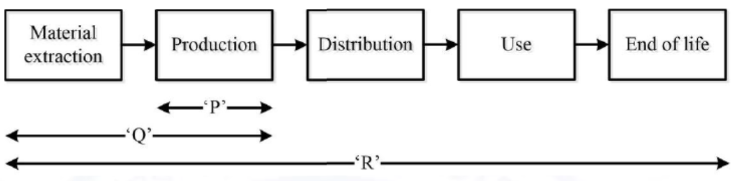
\includegraphics[width=0.75\columnwidth]{figs/image_4.png}
    \caption{Typical Phases of the life cycle of a product}
    \label{figure4}
\end{figure}
\begin{enumerate}
    \item 'R' represents cradle-to-grave analysis.
    \item 'P' represents cradle-to-gate analysis.
    \item 'Q' represents gate-to-grave analysis.
    \item 'R' represents gate-to-gate analysis.
\end{enumerate}

\item The United Nations Conference on Environment and Development was held in 1992 in Rio de Janeiro, Brazil. During this conference, several environmental management principles were adopted by many countries.\\ \\
Which one of the following principles allows the governments to take mitigation measures on the environmental issues having serious threats or irreversible damage, even if there is scientific uncertainty about such issues?
\hfill\brak{GATE~ES~2021}
\begin{enumerate}
    \item Polluters pay principle
    \item Precautionary priniciple
    \item Extended producer responsibility
    \item Common but differentiated responsibilities
\end{enumerate}

\item Choose the correct order of biodegradability (highest to lowest) of the following municipal solid waste components.
\hfill\brak{GATE~ES~2021}
\begin{enumerate}
    \item Food $>$ Newspaper $>$ Polyvinyl Chloride (PVC)
    \item Newspaper $>$ Food waste $>$ Polyvinyl Chloride (PVC)
    \item Food waste $>$ Polyvinyl Chloride (PVC) $>$ Newspaper
    \item Polyvinyl Chloride(PVC) $>$ Food waste $>$ Newspaper
\end{enumerate}

\item In proximate analysis, when a $10 kg$ moisture-free solid sample is heated in a furnace at $950\celsius$ in the \textit{absence} of air, its mass is reduced by $6 kg$. If the same $10 kg$ moisture-free solid sample is heated in the furnace at the same temperature in the \textit{presence} of air, its mass is reduced by $7 kg$. The percentage of fixed carbon in the sample is \_\_\_\_\_.
\hfill\brak{GATE~ES~2021}
\begin{enumerate}
    \item 20 \%
    \item 60 \%
    \item 10 \%
    \item 30 \%
\end{enumerate}

\item Chlorine is most effective as a water disinfectant at a pH of \_\_\_\_\_\_.
\hfill\brak{GATE~ES~2021}
\begin{enumerate}
    \item 6
    \item 8
    \item 10
    \item 12
\end{enumerate}

\item The oxidation states of $'N'$ in $NH_4^+, NO_2^- \text{and } NO$ are \_\_\_\_\_, respectively.
\hfill\brak{GATE~ES~2021}
\begin{enumerate}
    \item +2, -3, and +3
    \item -3, +3, and +2
    \item -3, +3, and -4
    \item +4, -2, and +2
\end{enumerate}

\item What is the pH of a water sample having $H^+$ concentration of $10 mg/L$? \\ The atomic weight of $H$ is $1 g/mol$.
\hfill\brak{GATE~ES~2021}
\begin{enumerate}
    \item 2
    \item 4
    \item 6
    \item 8
\end{enumerate}

\item Which of the following pairing of nucleotide bases is present in double helix DNA?
\hfill\brak{GATE~ES~2021}
\begin{enumerate}
    \item Thymine - Cystosine
    \item Adenine - Thymine
    \item Cytosine - Adenine
    \item Uracil - Thymine
\end{enumerate}

\item Which of the following is/are both greenhouse gas(es) and ozone depleting substance(s)?
\hfill\brak{GATE~ES~2021}
\begin{enumerate}
    \item $CFC-11$
    \item $CO_2$
    \item $HCFC-22$
    \item $N_2O$
\end{enumerate}

\item The ordinary differential equation\\ $\frac{dy}{dx} = x^2y$ \\ has $y$ as the dependent variable and $x$ as the independent variable. Which of the following classification(s) is/are applicable to the equation?
\hfill\brak{GATE~ES~2021}
\begin{enumerate}
    \item Linear
    \item Non-linear
    \item First order
    \item Second order
\end{enumerate}

\item Consider the following equation:
$$x^3-10x^2+31x-30 = 0$$
     Which of the following is/are the root(s) of the above equation?
\hfill\brak{GATE~ES~2021}
\begin{enumerate}
    \item 1
    \item 2
    \item 3
    \item 4
\end{enumerate}

\item A wind rose is a representation of meteorological conditions. Which of the follwing is.are included in this representation?
\hfill\brak{GATE~ES~2021}
\begin{enumerate}
    \item Mixing height
    \item Wind Speed
    \item Wind direction
    \item Percentage of time
\end{enumerate}
\bigskip

Q.23-Q.25 Numerical Answer Type(NAT), carry ONE mark each (no negative marks).
\\
\item A flocculation tank used for water treatment has a velocity gradient $(G)$ of $800 s^{-1}$. The volume of the tank is $40 m^3$. The dynamic viscosity of water is $9\times10^{-4} Ns/m^2$. The theoretical power required to maintain the given velocity gradient is \_\_\_\_\_\_ kW \textit{(rounded off to the nearest integer)}.
\hfill\brak{GATE~ES~2021}

\item In a sample, the growth of microbial cells started with an initial concentration of $5\times 10^4$ cells per millilitre ($mL$) of the sample. After a certain time period, the cell concentration was found to be $1280\times 10^4$ cells per $mL$ of the sample. Assuming binary fission of cells and no cell death, the number of generations of cell growth occurred in this time period is \_\_\_\_\_\_\_\_ \textit{(answer in integer)}.
\hfill\brak{GATE~ES~2021}

\item A water jet discharging from a $4 cm$ diameter orifice has a diameter of $3.5 cm$ at its vena contracta. The coefficient of velocity is defined as the ratio of the actual velocity of the jet at vena contracta to the theoretical velocity of the jet. If the coefficient of velocity is 0.98, the coefficient of discharge for the orifice will be \_\_\_\_\_\_\_ \textit{(rounded off to two decimal places)}. \hfill\brak{GATE~ES~2021}\\

Q.26-Q.34 Multiple Choice Question (MCQ), carry TWO mark each (for each wrong answer: -2/3). \\

\item The $2\times2$ matrices $P$ and $Q$ satisfy the following relations:\\
$P + Q = \myvec{3 & 1\\2 & 12}$ and \\ $P-Q = \myvec{-1 & -7\\8 & 2}$ \\ The matrix $Q$ is equal to \_\_\_\_\_\_. \hfill\brak{GATE~ES~2021}
\begin{enumerate}
    \item $\myvec{2 & 4\\-3 & 5}$
    \item $\myvec{1 & -3\\5 & 7}$
    \item $\myvec{2 & -3\\4 & 5}$
    \item $\myvec{1 & 0\\0 & 1}$
\end{enumerate}

\item A biased die has six faces numbered as $k=1,2,3,4,5,\text{and } 6.$ On rolling the die, the probability of the number $k$ appearing is proportional to $k^2$. What is the probability that an even number will appear on rolling the die? \hfill\brak{GATE~ES~2021}
\begin{enumerate}
    \item $\frac{35}{91}$
    \item $\frac{56}{91}$
    \item $\frac{12}{21}$
    \item $\frac{9}{21}$
\end{enumerate}

\item Match the entries in Column I with the correct entries in column II.
\hfill\brak{GATE~ES~2021}
\begin{table}[H]
\centering
\begin{tabular}{|l|l|}
\hline
\textbf{Column I} & \textbf{Column II} \\ \hline
P. Diffusion & (i) Pasquill \\ \hline
Q. Drag force & (ii) Fick \\ \hline
R. Atmospheric stability & (iii) Stokes \\ \hline
\end{tabular}
\end{table}
\begin{enumerate}
    \item P-(iii), Q-(ii), R-(ii), S-(i)
    \item P-(iv), Q-(ii), R-(iii), S-(i)
    \item P-(iii), Q-(i), R-(ii), S-(iv)
    \item P-(i), Q-(iii), R-(iv), S-(ii)
\end{enumerate}

\item Which of the following international multilateral agreements (conventions, protocols) from column I match with the entries in Column II?
\hfill\brak{GATE~ES~2021}
\begin{table}[H]
\centering
\renewcommand{\arraystretch}{1.3} % row height
\begin{tabular}{|l|l|}
\hline
Column I & Column II \\ \hline
P. Ramsar Convention & (i) Ozone depletion \\ \hline
Q. Kyoto Protocol & (ii) Trans-boundary movement of hazardous wastes \\ \hline
R. Basel Convention & (iii) Climate change \\ \hline
S. Montreal Protocol & (iv) Conservation of wetlands \\ \hline
\end{tabular}
\end{table}
\begin{enumerate}
    \item P-(iv), Q-(iii), R-(ii)
    \item P-(ii), Q-(i), R-(iii)
    \item P-(i), Q-(iii), R-(ii)
    \item P-(oo), Q-(iii), R-(i)
\end{enumerate}


\item An ideal PFR or an ideal CFSTR may be used to degrade a pollutant with first order reaction kinetics. Both the reactors are fed with the same inlet concentration and the same volumetric flow rate, and are designed to achieve the same outlet concentration. Which of the following statements is true when comparing PFR with CFSTR?\\

PFR is Plug Flow Reactor.\\

CFSTR is Continuous Flow Stirred Tank Reactor (also referred to as CSTR). \hfill\brak{GATE~ES~2021}
\begin{enumerate}
    \item PFR will always require less reactor volume than CFSTR.
    \item PFR will require the same reactor volume as CFSTR.
    \item CFSTR will always require less reactor volume than PFR.
    \item CFSTR can sometimes require less reactor volume than PFR.
\end{enumerate}

\item A $200 mL$ sample of water has an initial $pH = 9$. In order to determine alkalinity, the sample was titrated using $0.02 N$ $H_2SO_4$ acid to an end point of $pH = 4.5$. In the titration, $25 mL$ of $0.02 N$  $H_2SO_4$ acid was required. What is the total alkalinity of the sample in $mg/L$ as $NaHCO_3$?

[Atomic weight ($g/mol$): $Ca = 40, Na = 23, H = 1, C = 12, S = 32, \text{and } O = 16$]
\hfill\brak{GATE~ES~2021}
\begin{enumerate}
    \item 20
    \item 125
    \item 210
    \item 305
\end{enumerate}

\item A sewage treatment plant (STP) receives sewage at a flow rate of $20000 m^3$ per day. The sewage has $200 mg/L$ of suspended solids. Assume 60\% suspended solids are removed in the primary clarifier. The underflow (i.e. sludge) removed from the clarifier contains 5\% solids (by weight).\\
The daily volume of the sludge generated will be
\_\_\_\_\_\_\_ $m^3$ per day.\\
Assume sludge density $= 1000 kg/m^3$. \hfill\brak{GATE~ES~2021}
\begin{enumerate}
    \item 48
    \item 80
    \item 480
    \item 800
\end{enumerate}

\item In context of municipal solid waste treatment, match the equipment in List I with their function in List II. \hfill\brak{GATE~ES~2021}
\begin{table}[H]
\centering
\renewcommand{\arraystretch}{1.3} % row height
\begin{tabular}{|l|l|}
\hline
List I & List II \\ \hline
P. Trommel & (i) Size reduction \\ \hline
Q. Magnetic separator & (ii) Aluminium separation \\ \hline
R. Hammer mill & (iii) Screening \\ \hline
S. Eddy current separator & (iv) Ferrous metal recovery \\ \hline
\end{tabular}
\end{table}
\begin{enumerate}
    \item P-(iii), Q-(iv), R-(i), S-(ii)
    \item P-(iii), Q-(ii), R-(iv), S-(i)
    \item P-(i), Q-(iv), R-(iii), S-(ii)
    \item P-(iv), Q-(ii), R-(i), S-(iii)

\end{enumerate}

\item The characteristics of a water sample are as follows: $Na^+ = 92$ $mg/L$, $K^+ = 19.5$ $mg/L$, $Ca^{2+} = 40$ $mg/L$, and $Mg^{2+} = 24$ $mg/L$. What is the sodium adsorption ratio (SAR) of the water sample which may be considered for irrigation purposes?\\
Atomic weight ($g/mol$): $Na = 23$, $K = 39$, $Ca = 40$, and $Mg = 24$. \hfill\brak{GATE~ES~2021}
\begin{enumerate}
    \item 2.83
    \item 1.94
    \item 2.00
    \item 4.00
\end{enumerate}
\bigskip

Q.35-Q.40 Multiple Select Question (MSQ), carry TWO mark each (no negative marks).\\

\item Which of the following is true for the nitrifying bacteria belonging to genus \textit{Nitrobacter}? \hfill\brak{GATE~ES~2021}
\begin{enumerate}
    \item They are autotrophs.
    \item They are eukaryotes.
    \item They convert chemical energy to cellular energy using mitochondria.
    \item They convert $NO_3^-$ to $NO_2^-$.
\end{enumerate}

\item Which of the following is/are the dominant mechanism(s) for the renoval of spherical particles with diameter less than $10 \mu m$ from a gas stream using a fabric filter? \hfill\brak{GATE~ES~2021}
\begin{enumerate}
    \item Impaction
    \item Gravitation
    \item Interception
    \item Diffusion
\end{enumerate}

\item In air pollutio, which of the following is/are classified as \textit{primary} pollutants? \hfill\brak{GATE~ES~2021}
\begin{enumerate}
    \item Carbon Monoxide ($CO$)
    \item Sulphur dioxide ($SO_2$)
    \item Ozone ($O_3$)
    \item  Nitrogen dioxide ($NO_2$)
\end{enumerate}

\item Which of the following is/are correct for the process of glycolysis? \hfill\brak{GATE~ES~2021}
\begin{enumerate}
    \item There is net decrease in standard Gibbs free energy
    \item The end product is glyceraldehyde 3-phosphate.
    \item First phase includes the phosphorylation of the glucose molecule.
    \item It results in the net gain of NADH.
\end{enumerate}

\item In the context of water quality, which of the following is/are correct for the most probable number (MPN) of a water sample? \hfill\brak{GATE~ES~2021}
\begin{enumerate}
    \item The estimated organisms are gram negative,
    \item It is based on the assumption of Poisson distribution.
    \item It measures the exact number of microorganisms present in the sample.
    \item It includes the quantification of pathogenic virus.
\end{enumerate}

\item For any particular location, which of the following would influence the solar radiation incident on a rooftop solar water heater? \hfill\brak{GATE~ES~2021}
\begin{enumerate}
    \item Heater surface temperature
    \item Day of the year
    \item Hot water temperature
    \item Sky clearness
\end{enumerate}
\bigskip 

Q.41-Q.55 Numerical Answer Type (NAT), carry TWO mark each (no negative marks). \\

\item If $f(x) + 3f(g(x))=x-2$, \\ where $g(x)=\frac{3x+1}{x-3}$, \\ then the value of the ratio $\frac{f(5)}{f(8)}$ is \_\_\_\_\_\_ \textit{(answer in integer)}. \hfill\brak{GATE~ES~2021}

\item Consider a funtion $y=f(x)$ which satisfies the following equation:\\ $\frac{d^2y}{dx^2}-\frac{dy}{dx}=0$\\ As $x\to-\infty, y=1,$ and at $x=0,y=2$.\\ The value of $\frac{dy}{dx}$ at $x=0$ is \_\_\_\_\_\_ \textit{(answer in integer)}. \hfill\brak{GATE~ES~2021}

\item The concentration of $NO_2$ in the air at NTP is reported as 0.30 ppmv (ppm by volume). The concentration of $NO_2$ in $\mu g/m^3$ is \_\_\_\_\_\_ \textit{(rounded off to the nearest integer)}.\\

[At NTP, temperature = $298K$, pressure = $1 atm$, and one mole of ideal gas occupies $24.45 L$]

[Molecular weight of $NO_2$ = $46 g/mol$] \hfill\brak{GATE~ES~2021}

\item In open channel flow, the specific energy is the total energy per unit weight of a liquid, where the component potential energy is measured from the bed of the channel as the datum.\\
A rectangular channel of $10m$ width carries $20 m^3/s$ of water. The depth of flowing water is $1 m$. The specific energy for this flow condition is \_\_\_\_\_\_ $m$ \textit{(rounded off to one decimal place)}.\\ 

Consider acceleration due to gravity $(g)$ = $10 m/s^2$. \hfill\brak{GATE~ES~2021}

\item Two reservoirs are connected by a pipeline consisting of two pipes $'A'$ and $'B'$ in series. The two pipes are of same length and have the same Darcy friction factor. If the internal diameter of pipe $'B'$ is twice as large as the internal diameter of pipe $'A'$, the ratio of the head loss in pipe $'A'$ to that in pipe $'B'$ is \_\_\_\_\_\_ \textit{(answer in integer)}. Neglect all minor losses. \hfill\brak{GATE~ES~2021}

\item In a field test of a geological formation of permeable soil (porosity = 20\%), the hydraulic gradient was found to be 2\%. The actual seepage velocity of the flow was found to be $0.0025 m/s$. Assume that the flow is in the laminar regime. The permeability$(K)$ of the aquifer is \_\_\_\_\_\_ $m/s$ \textit{(rounded off to three decimal places)}. \hfill\brak{GATE~ES~2021}

\item An underground hazardous waste storage tank is leaking. The contaminant concentration directly beneath the site is $0.5 mg/L$. The contaminant is travelling at an effective rate of 0.4 m per day towards a water well which is $2 km$ away.\\
Assume that the degradation of the contaminant follows a first order reaction, and the initial concentration of the contaminant becomes half in 10 years.\\
In this case, the contaminant concentration expected at the well under steady state conditions is \_\_\_\_\_\_\_ $mg/L$ \textit{(rounded off to two decimal places)}. \hfill\brak{GATE~ES~2021}

\item The net profit expected from a manufacturing unit is \rupee $6000$ per year. The operational life of the unit is 15 years. Assuming a fixed discount rate of 8\% per annum, the net present worth of the profit earned over the operational life is \rupee \_\_\_\_\_\_ \textit{(answer in integer)}. \hfill\brak{GATE~ES~2021}

\item A $900 mm$ internal diameter sewer is laid at a slope of 0.004 and has an actual flow of $ 0.15 m^3/s$. Assuming Manning's roughness coefficient to be 0.013, the ratio of the actual flow to the flow when the sewer is running full is \_\_\_\_\_\_ \textit{(rounded off to two decimal places)}.\\
Take $\pi=3.14$. \hfill\brak{GATE~ES~2021}

\item A 10 million litres per day (MLD) sewage treatment plant (STP) is based on the Activated Sludge Process (ASP). First, the sewage undergoes primary treatment and the resulting treated sewage has $BOD_5$ of $140 mg/L$ concentration. This is further passed through a $1500 m^3$ capacity aeration tank (in ASP), where the mixed liquor volatile suspended solids (MLVSS) concentration is maintained at $3000 mg/L$. The concentration of $BOD_5$ of the treated sewage is $5 mg/L$.\\
The Food to Microorganisms ratio (F/M) of the ASP is \_\_\_\_\_ $day^{-1}$ \textit{(rounded off to two decimal places)}. \hfill\brak{GATE~ES~2021}

\item The municipal solid waste (MSW) generated in a community (population = 100000) is disposed on a $12\times10^4 m^2$ landfill site, which can be filled to a total depth of $25 m$ (including soil cover). Assume that MSW is generated at a rate of $2.5 kg$ per person per day and its compacted density is $800 kg/m^3$. If the volumetric ratio of MSW and soil cover is 5:1, the useful life of the landfill site is \_\_\_\_\_
years \textit{(rounded off to the nearest integer)}. \hfill\brak{GATE~ES~2021}

\item A mechanized stationary container system is proposed for waste collection from a commercial area. The container unloading time is 0.1 hours per container. There are two containers at each location and the drive time between the two locations is 0.2 hours. The maximum waste 'pick-up time' is 2.4 hours per trip.

The 'pick-up time' starts at the instant the truck arrives at the first pick-up location and ends when the last container on the route is emptied. The maximum number of locations which can be covered in a trip by the collection vehicle are \_\_\_\_\_\_ \textit{(answer in integer)}. \hfill\brak{GATE~ES~2021}

\item The molar concentrations $(M, i.e. mol/L)$ of some ionic species in a water sample were estimated as follows:

$Na^+ = 0.25 M$; $Ca^{2+} = 0.12 M$; $Cl^- = 0.32 M$;$HCO_3^-= 0.05 M$.

The ionic strength of this water sample is \_\_\_\_\_ $M$ \textit{(up to two decimal places)}. \hfill\brak{GATE~ES~2021}

\item Excess amount of solid calcium sulphate $(CaSO_4)$ was added to a pure water sample ($pH = 7$) so that some solids remain undissolved at the equilibrium. The solubility product of $CaSO_4$ is $2\times10^{-5} mol^2/L^2$. The molar concentration of $SO_4^{2-}$ in this water sample at equilibrium will be \_\_\_\_\_\_ $mol/L$ \textit{(rounded off to three decimal places)}. \hfill\brak{GATE~ES~2021}

\item A facultative pond system for sewage treatment consists of two ponds in series. The hydraulic retention time (HRT) of each pond is 6 days. The total $BOD_5$ reduction through the entire pond system is 90\%. If the ponds are considered to be completely mixed, then the rate constant describing the $BOD_5$ removal is \_\_\_\_\_\_ $day^{-1}$ \textit{(rounded off to two decimal points)}. Assume that the rate constant is same for both the ponds. \hfill\brak{GATE~ES~2021}

\end{enumerate}
\bigskip
\begin{center}
    \textbf{END OF THE QUESTION PAPER}
\end{center}
\end{document}